\chapter{Metodologia}
O software desenvolvido tem como objetivo demonstrar uma solução para o problema de PRVJT, descobrindo caminho viáveis entres diferentes endereços, onde é possível realizar as entregas em um período pre determinado, também identificar roteiros que são impossíveis de serem realizados a tempo. 

Para adquirir informações próximas as reais de distancia e locomoção entre endereços esta sendo utilizado a API do Google Maps\cite{GoogleMatrix}.

Por se tratar de entregas de pequenos porte, os testes foram criados com endereços dentro das proximidades da cidade de São Paulo, uma grande metrópoles com um dos maiores índices de transito \cite{TomTom}, por esse motivo a menor distância de rota pode não ser a melhor escolha para certos horários do dia, podendo uma rota com maior distância que evita transito ser uma melhor escolha.

Para preparar o calculo da rota, deve-se levar em consideração que todos os entregadores partem de uma única origem chamada deposito, a quantidade de entregadores é predefinida, o sistema ira devolver rotas para atender todos os pontos visando diminuir a quantidade necessária de entregadores e distancia percorrida sem desrespeitar as restrições de janelas de tempo.

Cada entrega tem um tempo médio de descarga, produtos pequenos podem demorar minutos, muitos produtos demoram mais para a retirar do veiculo e produtos grande podem precisar ser levamos com mais cuidado.

Cada endereço tem um horário de abertura e fechamento para realizar entregas, por exemplo, um super mercado recebe produtos na madrugada, já que receber em seu horário normal de abertura provavelmente irá atrapalhar as compras dos clientes, então esse horário deve ser considerado como restrição de tempo.

Por causa das restrições de tempo, quando um entregador chega a um endereço deve ser avaliado com penalidade caso o mesmo chegue antes ou depois da janela de tempo, se chegar antes o mesmo deve esperar até o horário de abertura do endereço, somar o tempo de descarga e sair para o próximo endereço,  caso chegue depois é considerado que não é uma solução de rota viável para as restrições definidas. 

É importante avaliar situações onde não é possível realizar as entregas, essas situação podem depender de distancia, por exemplo, caso o deposito esteja longe a ponto de um entregador não ter como chegar no endereço dentro de sua janela de tempo, ou caso mesmo sendo próximos ocorrer uma mudança no transito tornando impossível realizar a entrega á tempo, ou ainda pelo fato de ser definido um numero finito de entregadores, que podem não ser suficientes para realizar todas as entregas do roteiro.

Depois que uma entrega é feita, uma nova rota deve ser recalculada, agora como ponto inicial o endereço atual, todo o processo será refeito para verificar se o transito ou possível atrasos não afetaram a ordem dos próximos destinos, depois do recalculo o entregador deve seria o próximo destino indicado.

Se caso não for mais possível entregar no horário por motivos de piora de transito ou um grande tempo de atraso para descarregar, um alerta será emitido indicando que todos os destinos não podem ser visitados a tempo.

Cada entregador tem seu próprio recalculo de rota, sendo que se um entregador concluir todos os destinos, os outros continuam pedindo novas rotas até que todos terminem suas entregas.

O fluxograma a baixo demostra o fluxo da solução.

\begin{center}
    \makebox[\linewidth]{
        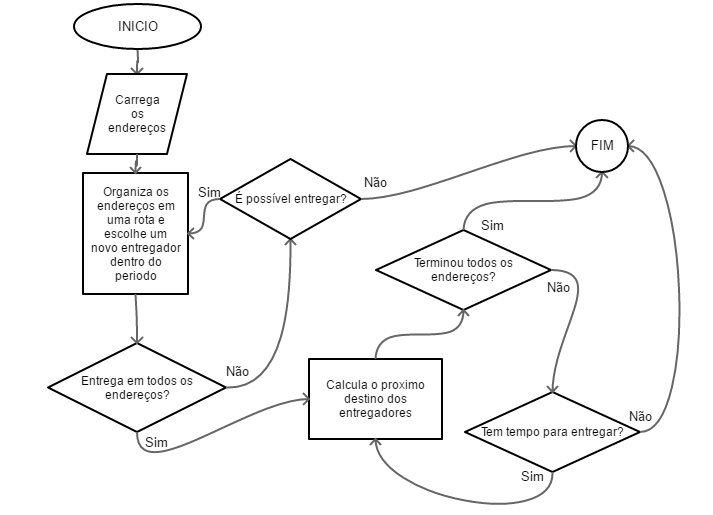
\includegraphics[keepaspectratio=true,scale=0.6]{ibagens/Fluxograma.png}}
    \captionof{figure}{Fluxograma macro do funcionamento do software.  }
    \label{fig:FluxoSoftware}
\end{center}

Sempre que é necessário calcular a rota, o modulo de GA é chamado. Considerando que um individuo é uma solução completa, gera uma população de varias soluções, onde a ordem da rota é aleatória somente mantendo o deposito fixo como primeiro endereço para criar a população inicial.

Para cada rota da população de indivíduos a seleção determina dois para a realização do cruzamento, onde endereços das duas rotas são trocados de forma a criar duas novas rotas mantendo o deposito sempre como inicial. A mutação é executada individual em cada rota, mudando de posição um ou mais endereços da rota, sempre mantendo o deposito como ponto inicial.

Depois que todas as rotas dos indivíduos da população foram modificados, agora é hora de verificar quais são os melhores, o que define isso é a função de aptidão, todos os parâmetros da rota são agrupados em um único numero e a rota que tem o menor número é a melhor rota da população. O valor de aptidão é definido com a soma da distância entre todos os endereços da rota, mais o tempo de cada um dos trajetos com o tempo de espera e descarga.

A função de aptidão do GA considera para uma frota homogênea de \textit{m} veículos o horário de saída como parâmetros inicial, com isso, utiliza o tempo dado pelo Google Maps entre os pontos e soma ao horário verificando se está dentro da janela de tempo do destino. Se o horário calculo for menor que o de abertura, é somado o tempo restante de espera e uma penalidade por chegar antes. Se o horário for maior que o tempo de fechamento, é somado o tempo restante de espera até a abertura no próximo dia mais uma penalidade pela diferença. O Valor de aptidão final é a soma da distancia em metros do percurso passando por todos os pontos, com o tempo total em minutos com as penalidades de chegar antes ou depois das janelas de tempo.

A função de aptidão é definida como:

\begin{center}
	\makebox[\linewidth]{
		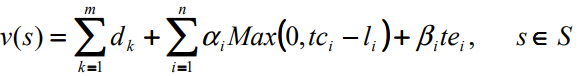
\includegraphics[keepaspectratio=true]{ibagens/aptidao.png}}
	\captionof{figure}{Formula de avaliação de solução de rota \cite{Gendreau2} }
	\label{fig:MetodoAptidao}
\end{center}

Onde para cada ponto de entrega \textit{i} temos um \(e_i\)
e um \(li\)  que representam, respectivamente, a abertura e o fechamento
da janela de tempo do ponto \textit{i}, O \(tc_i\) é o tempo de chegada do veículo no ponto \(i\), \(te_i\) calculado como \(e_i - tc_i\). 

\(dk\) é a distância total percorrida na rota $k$ para todo $k=1,...,m$, \(\alpha_i\) é o coeficiente de penalidade associado à chegada do veículo no vértice $i$ após o fechamento da janela de tempo.

Para seção utilizamos o operador \textbf{Selection Roulette Wheel}, onde é feita uma soma de todos os valores da função de aptidão da população, depois calculado a porcentagem de cada indivíduo referente ao total e guardada em um vetor. Então é gerado um valor $X$ aleatório entre 0 e 1, e multiplicado pelo valor total dos pesos. 
Para selecionar o indivíduo é feito um loop no vetor de pesos e seus valores somados até que seja menor ou igual ao valor $X$, a posição atual no vetor deste valor será o utilizada para selecionar o individuo no vector de indivíduos. 
Desta forma aumentando a possibilidade de selecionar um indivíduo com melhor aptidão.

O cromossomo deve especificar a quantidade de veículos/entregadores necessários, como as demandas são particionadas entre esses veículos e qual rota cada veiculo deve fazer. Adotamos uma representação onde o material genético de um individual contém várias rotas, cada uma delas composta por um subconjunto ordenado de clientes \ref{fig:genoma}. Todas as demandas pertencentes ao problema a ser resolvido devem estar presentes na combinação dessas rotas. Aonde cada uma inicia e finaliza no deposito \ref{fig{genoma_rotas}}

\begin{center}
	\makebox[\linewidth]{
		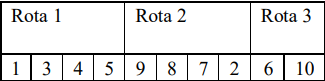
\includegraphics[keepaspectratio=true]{ibagens/genoma.png}}
	\captionof{figure}{Representação geral do genoman}
	\label{fig:genoma}
\end{center}

\begin{center}
	\makebox[\linewidth]{
		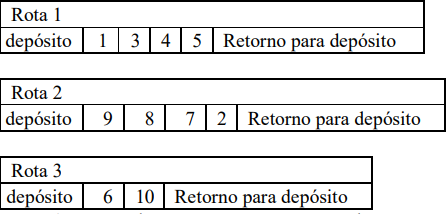
\includegraphics[keepaspectratio=true]{ibagens/genoma-rotas.png}}
	\captionof{figure}{Representação do genoma separando rotas}
	\label{fig:genoma_rotas}
\end{center}

Para cruzamento foi escolhido o operador proposto por \cite{Pereira_Tavares} que teve resultados positivos para o PRV puro, o operador por si só não promove uma troca mútua de material genético entre dois pais. Em vez disso, quando submetidos a essa operação, um indivíduo recebe um fragmento de material genético (mais precisamente, uma sub-rota) de outro pai e insere-o em uma de suas próprias rotas. O doador não é modificado. A localização geográfica dos clientes é usada para determinar a posição onde a sub-rota é inserida, de forma a ser inserida no ponto mais próximo ao primeiro ponto da sub-rota e que não pertença a ela. A definição do algoritmo pode ser verificada em \ref{algcx_alg}.

\begin{algorithm}
	\SetKwInOut{Input}{Entrada}
	\SetKwInOut{Output}{Saida}
	   
	\underline{Função Cruzamento} $(I_1,I_2)$\;
	\Input{Dois indivíduos da população $I_1$ e $I_2$}
	\Output{Um descendente $I_d$}
	\BlankLine
	$SR \leftarrow $ Do material genético de $I_2$, selecione  aleatoriamente uma sub-rota \{$a_1, a_2,…, a_n$\}
	
	$C \leftarrow $ Encontre o cliente geograficamente mais próximo de $a_1$ não pertencente a $SR$
		
	Insira $SR$ no material genético de $I_1$ de maneira que $a_1$ seja
	colocado imediatamente após $C$

	
	Do material genético original de $I_1$, remover todos os 
	clientes duplicados que também aparecem em $SR$, obtendo um descendente $I_d$ 
	
	\nl\KwRet{$I_d$}

	\caption{Algoritmo de cruzamento aplicado a PRV}\label{algcx_alg}
\end{algorithm}

O exemplo da figura \ref{fig:cx_alg} ajuda a ilustrar como o cruzamento atua. Assume-se que o cliente 6 é o que está geograficamente mais próximo do cliente 9. Desta forma, a sub-rota
\{9, 1, 10\} é selecionado de $I_2$ e é inserido em uma das rotas de $I_1$, imediatamente após o 6. O operador de cruzamento possibilita que um fragmento de informação que faz parte de um indivíduo possa ser incorporado em outra solução. Dada a seu comportamento, ele não pode adicionar novos veículos à solução. Por outro lado, pode acabar por remove-los.

\begin{center}
	\makebox[\linewidth]{
		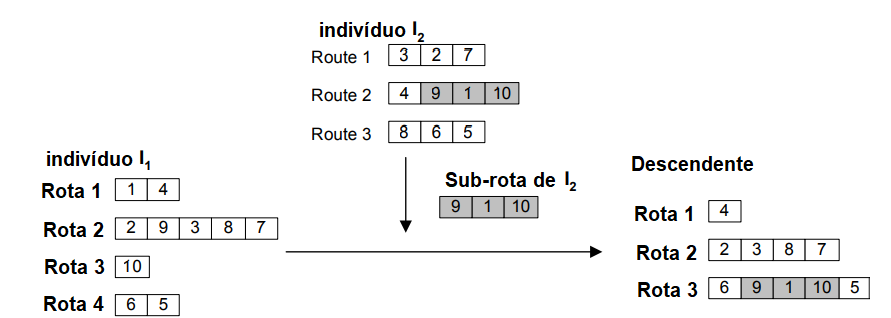
\includegraphics[keepaspectratio=true,scale=0.8]{ibagens/cx_alg.png}}
	\captionof{figure}{Exemplo de Cruzamento, adaptado de \cite{Pereira_Tavares}}
	\label{fig:cx_alg}
\end{center}


Porem no caso de nossa implementação ao fazer a seleção de um par de de indivíduos \textit{(a,b)} para o cruzamento, geramos um par de descendentes \textit{({x,y})}, de forma que \(x = a \rightarrow b\) e \(y = b \rightarrow a\) aonde $x \rightarrow y$ implica na operação de cruzamento aplicado de $x$ em $y$.


Descendentes resultantes do cruzamento podem estar sujeitos a mutação. Nós consideramos 4 operadores de mutação comuns de serem aplicados em representações \textit{Baseadas em ordem}. \cite{Rocha}. Estes são:

\textbf{Swap}: Seleciona dois clientes de forma aleatória e os troca. Os clientes selecionados podem pertencer a mesma ou não.

\textbf{Inversion}: Seleciona uma sub-rota de forma aleatória e inverte a ordem de visita aos clientes pertencentes a ela.

\textbf{Insertion}: Seleciona aleatoriamente um cliente e o insere em outro lugar. A rota onde este será inserido é escolhida aleatoriamente. É possível criar uma nova rota com novo entregador para este cliente. Nos experimentos deste trabalho, a probabilidade de criar um novo rota é $1 / (2 \times V)$, onde $V$ representa o número de veículos da solução atual. Desta forma, a probabilidade de criar uma nova rota é inversamente proporcional à número de veículos já utilizados. 

Na figura \ref{fig:mt_alg}, mostramos um exemplo dessa operação.

\textbf{Displacement}: Seleciona aleatoriamente uma sub-rota e a insere em outro lugar. Este operador pode realizar intra ou inter deslocamento (se a sub-rota selecionada é inserida na
mesma ou em outra rota). Assim como no operador anterior, também é possível criar uma nova rota com a sub-rota (a probabilidade desta ocorrência é calculada da mesma forma).

\begin{center}
	\makebox[\linewidth]{
		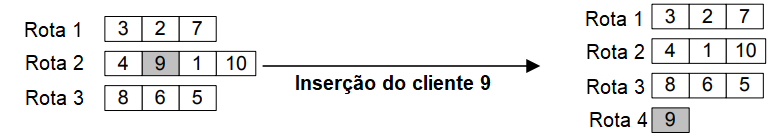
\includegraphics[keepaspectratio=true,scale=0.8]{ibagens/mt_alg.png}}
	\captionof{figure}{Exemplo de mutação, adaptado de \cite{Pereira_Tavares}}
	\label{fig:mt_alg}
\end{center}


\textit{Swap} e \textit{Inversion} não alteram o número de rotas de um indivíduo. Já \textit{Insertion} e \textit{Displacement} têm a capacidade de remover e adicionar veículos nos indivíduos.

Foi implementada  uma logica de elitismo simples, aonde uma próxima geração leva junto $N$ mais bem avaliados indivíduos da ultima geração.

O GA foi configurado com o numero de gerações em 200, tamanho da população em 1000, melhores indivíduos por geração em 20, com elitismo em 2 indivíduos, probabilidade de cruzamento em 70\% e de Mutação em 5\%.

Os testes foram configurados com um numero de 6 roteiros diferentes, endereços dentro da cidade de São Paulo e cidades próximas.

Considerando o transito médio enviado pelo Google Maps, para poder demostrar o impacto do transito nos caminhos calculados.
Tudo será rodado 10 vezes e será retirada uma média do valor de aptidão, por que, cada vez que roda o GA a resposta da solução pode mudar, por ele não ser determinístico.

E uma base pré-definidas rotas, para prevenir possíveis problemas sera ignorado o transito atual. Ja que o mesmo altera dependendo das condições do clima ou horário do dia. Então utilizando o Google Maps, um cache inicial foi preparado e o software utiliza simulando uma buscar ao Google Maps, com isso, a informação é obtida mais rapidamente e sempre fixa para garantir a resposta pré-determinada do teste.

O fluxograma a baixo demostra o funcionamento do software utilizando o GA.

\begin{center}
	\makebox[\linewidth]{
		\includegraphics[keepaspectratio=true]{ibagens/GA.png}}
	\captionof{figure}{Fluxograma macro da integração com o GA.}
	\label{fig:FluxoGA}
\end{center}

\chapter{Implementação}
 
Nesse capitulo será apresentado mais aprofundadamente as tecnologias, ferramentas e métodos que foram utilizados para a implementação do algoritmo genético para busca de rota com janela de tempo.

\section{Tecnologias}

O software foi desenvolvido na linguagem C\# com Visual Studio 2017 com o Framework  .Net Core 2.2 compatível com Windows, Linux e MacOs.
Foi desenvolvido uma WeApi em ASP.NET para consumo de uma pagina desenvolvida utilizando  ReactJS. Toda comunicação entre frontend e backend foi desenvolvida utilizando os conceitos de REST.

Também foi desenvolvido uma ferramenta para gravar os resultados obtidos pelo GA, porem este obtém as configurações de busca a partir de arquivos que contém os endereços e quantidade de entregadores.

Todos os testes presentes nesse trabalho foram obtidos rodando os testes em um computador I7 2600 de 3.4Ghz com 12GB de memória RAM.


\section{Estrutura do Projeto}

Para facilitar o entendimento inicial do projeto, é importante ter uma orientação de onde está cada parte de seu comportamento. A Software é divido em 4 projetos principais, sendo um projeto feito em ReactJS e 3  projetos em C\#, onde eles são:

\subsection{Calculador de Rotas - CalcRoute}

Projeto principal que tem toda a logica de preparação das rotas, recebendo parâmetros e utilizando o GA para gerar a resposta.
A classe PRVJTFinder que é responsável por essa tarefa, podendo carrega as configurações por arquivo ou recendo os parâmetros diretamente. Os endereços não precisam vim com as coordenadas, e sim apenas o nome, por que existe uma preparação dos endereços antes de começar o calculo das rotas que busca as coordenadas de cada endereço. Os projetos CalcRoute.GeneticAlgorithm e CalcRoute.Routes são auxiliares para o calculo da rota.

A interação com a API do Google Mapas é encontrada no projeto CalcRoute.Routes, ela permite 3 tipos de transito possíveis para o calculo de tempo entre as rotas, esses são:
\begin{itemize}
	\item Média considera a média historia entre os endereços.
	\item Otimista considera o melhor resultado histórico entre os endereços.
	\item Pessimista considera o pior resultado histórico entre os endereços.
\end{itemize}

\subsection{Gerador de Dados - CalcRoute.RouteGenerate}

Para ajudar na identificação dos melhores parâmetros a ser utilizado, esse projeto é configurado para utilizar todos os cruzamentos e mutação do GA, com isso, diferentes configurações de população, numero de gerações,taxa de cruzamento e taxa de mutação, podem ser testados e os resultados são agrupados em um arquivo CSV com o valor do melhor valor de aptidão encontrado para cada parâmetro para facilitar a analise dos dados.

\begin{center}
	\makebox[\linewidth]{
		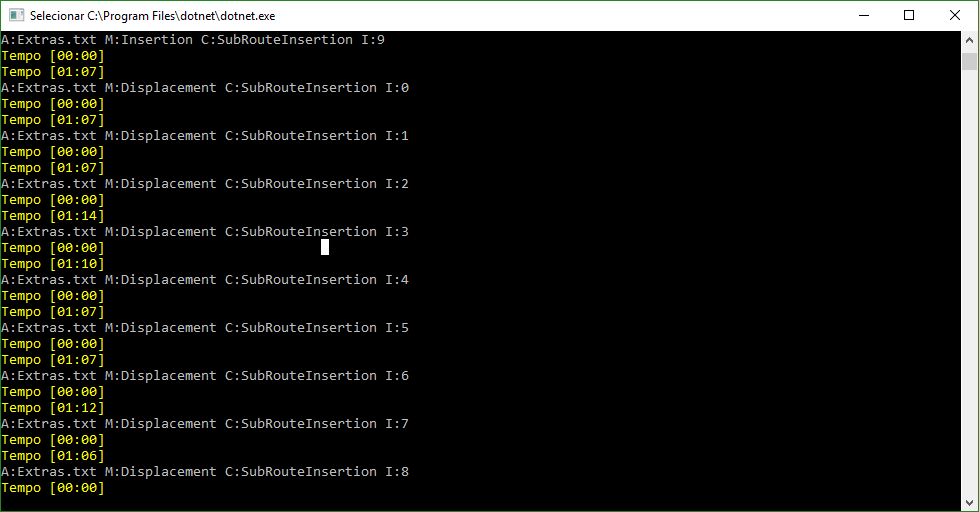
\includegraphics[keepaspectratio=true,scale=0.5]{ibagens/DataGenerate.png}}
	\captionof{figure}{Tela da geração de dados de comparação}
	\label{fig:DataGenerate}
\end{center}

\subsection{API de Calculo de Rotas - CalcRoute.API}

Projeto de comunicação com a interface usando POST, recebendo parâmetros da interface e organiza para serem calculados no CalcRoute. 
O retorno é organizado e os campos formatados para melhor apresentação na tabela da interface.

\subsection{Interface para comunicação com a API}

A interface é utilizada para interagir com o calculador de rotas de uma forma mais simples, podendo procurar por endereços, adicionar a lista, definir o deposito, os horários de cada endereço, numero de entregadores e tempo de descarga de cada endereço. Para melhor visualização dos testes, é possível encontrar todos os roteiros de teste para fácil execução e verifica os resultados.

\begin{center}
	\makebox[\linewidth]{
		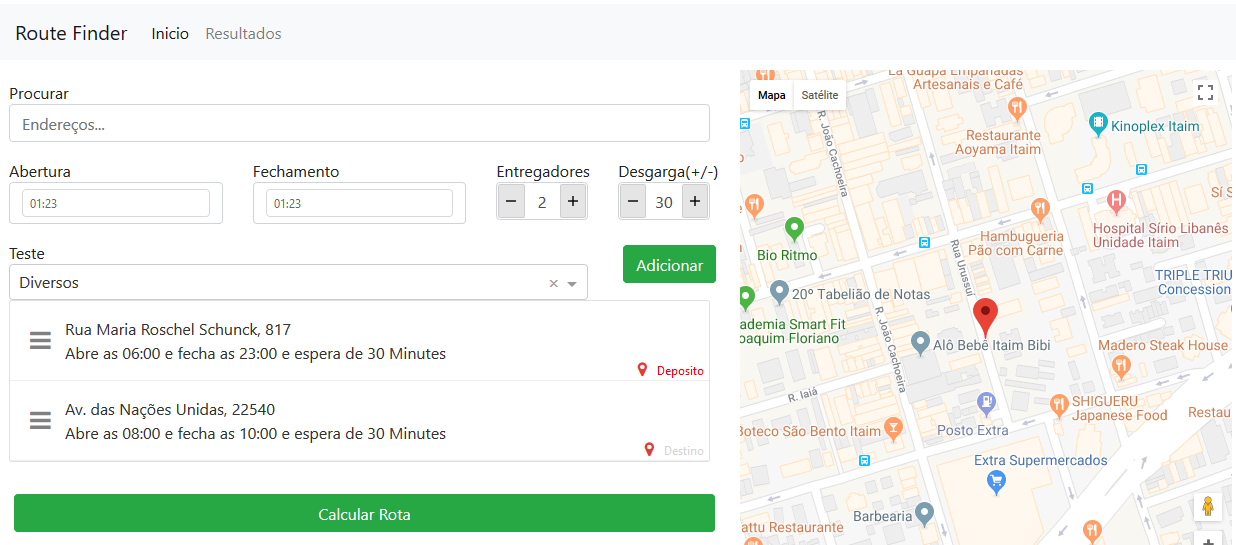
\includegraphics[keepaspectratio=true,scale=0.5]{ibagens/Interface.png}}
	\captionof{figure}{Aparência da interface, configuração das rotas}
	\label{fig:Interface}
\end{center}

\begin{itemize}
	\item No campo procurar é preciso digitar o endereço para ser localizado no Google Maps, uma lista de possíveis escolhas aparece a baixo assim que começa a digitar, encontra o endereço e selecione.
	\item O mapa exibe o endereço selecionado.
	\item Abertura é o horário que que é permitida a entrada no local, no caso do deposito é o horário que o entregador sai para realizar as entregas.
	\item Fechamento é o horário limite para realizar a entrega, no caso do deposito, é o horário limite para terminar todas as entregas, horário que o deposito fecha.
	\item Entregadores é o numero de entregados disponível para realizar as entregas.
	\item Descarga o tempo médio para descarregar no endereço de entrega, no caso do deposito esse campo não é utilizado.
	\item Adicionar Agrupa os campos do endereço, abertura, fechamento e descarga para a lista.
	\item Lista de endereços reúne todos os endereços escolhidos para enviar para o calculador de rotas, o primeiro da lista é sempre o deposito
	\item Calcular Rota faz a chama da Api de calculo e envia a lista.
\end{itemize}

\subsubsection{Configurações Avançadas}
As Configurações Avançadas ajudam no teste, podem definir configurações e fazer comparações de uma maneira mais ágil.
\begin{itemize}
	\item Usar Cache guarda as rotas carregar do google mapas para a primeira chamada e utiliza para as próximas consultas iguais.
	\item Tráfego configura a maneira que o Google Mapas trabalha com o trânsito, com as opção média, Otimista e Pessimista.
	\item Mutação define qual mutação deve ser utilizada no GA.
	\item Gerações define o numero de gerações que o GA deve rodar antes de retornar o melhor resultado encontrado.
	\item População define o tamanho população que o GA vai utilizar para calcular as rotas.
\end{itemize}

\begin{center}
	\makebox[\linewidth]{
		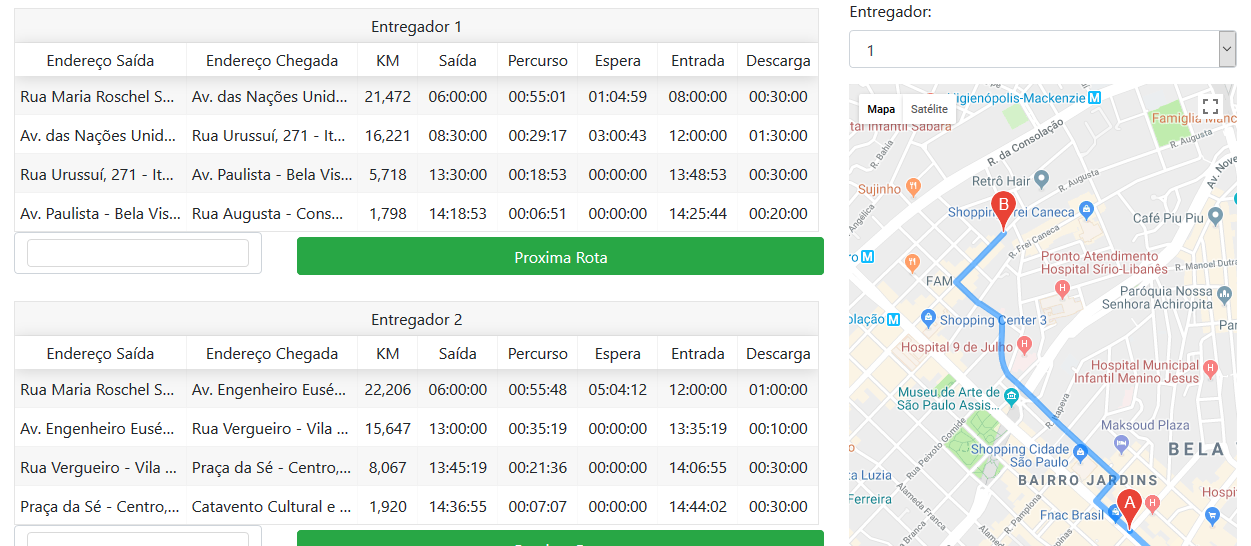
\includegraphics[keepaspectratio=true,scale=0.5]{ibagens/InterfaceResultado.png}}
	\captionof{figure}{Aparência da interface para exibição dos resultados}
	\label{fig:InterfaceResultado}
\end{center}

Cada entregador é exibido de forma separada, com sua própria tabela de endereço e recalculo para o próximo destino. A lista acima do mapa, é possível escolher qual rota será exibida no mapa, trocando entre os entregadores.
A tabela tem 8 colunas com informações de cada percurso, essa colunas são:
\begin{itemize}
	\item Endereço Saída: É o endereço que o entregador vai sair, na primeira vez será do deposito. Todos entregadores saem do mesmo endereço de deposito.
	\item Endereço Chegada: Endereço que o entregador chegará depois que sair do endereço de saída.
	\item KM: É a distancia em Quilômetros de cada percurso indicada pelo Google Maps.
	\item Saída: Horário que o entregador sairá para realizar a entrega.
	\item Percurso: Tempo de locomoção para chegar até o destino de entrega.
	\item Espera: Se chegar no destino antes do horário de abertura, esse é o tempo que o entregador ficará esperando.
	\item Entrada: Horário que o entregador consegui entrar para começar a realizar a descarga da entrega.
	\item Descarga: Tempo Médio para descarregador toda a encomenda.
\end{itemize}
Depois de finalizar a entrega o campo saída deve ser preenchido com o horário que está tudo pronto para fazer a próxima entrega e clicar no botão Próxima Rota, uma nova chamada para a API será feita somente com o entregador pedido, esse processo pode ser repetido até que todas os endereços sejam visitados.
